% Source: Code/xband-radar-sim/docs/radar_simulation_technical.tex
% Description: High-level simulation pipeline. The ray-to-compress loop executes 720 times (once per azimuth).

\documentclass[border=4pt]{standalone}
\usepackage{algpseudocode}
\usepackage{amsmath,amssymb,amsfonts}
\usepackage[T1]{fontenc}
\usepackage{graphicx}
\usepackage{pgfplots}
\usepackage{tikz}
\usepackage{xcolor}
\pgfplotsset{compat=1.18}
\usetikzlibrary{arrows.meta,positioning,shapes.geometric,calc,patterns,decorations.pathmorphing,3d,angles,quotes}

\definecolor{radargreen}{RGB}{0,255,0}
\definecolor{raycolor}{RGB}{255,165,0}
\definecolor{targetcolor}{RGB}{255,0,0}
\definecolor{groundcolor}{RGB}{139,90,43}
\definecolor{skycolor}{RGB}{135,206,235}
\definecolor{beamcolor}{RGB}{255,255,0}


\begin{document}
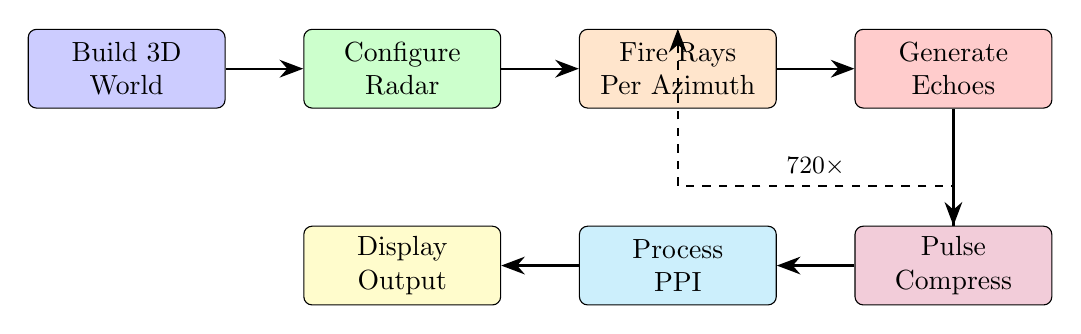
\begin{tikzpicture}[
    box/.style={rectangle, draw, minimum width=2.5cm, minimum height=1cm, align=center, rounded corners=3pt},
    arrow/.style={-{Stealth[length=3mm]}, thick}
]
    % Main pipeline boxes
    \node[box, fill=blue!20] (world) at (0,0) {Build 3D\\World};
    \node[box, fill=green!20] (config) at (3.5,0) {Configure\\Radar};
    \node[box, fill=orange!20] (rays) at (7,0) {Fire Rays\\Per Azimuth};
    \node[box, fill=red!20] (signal) at (10.5,0) {Generate\\Echoes};

    \node[box, fill=purple!20] (compress) at (10.5,-2.5) {Pulse\\Compress};
    \node[box, fill=cyan!20] (ppi) at (7,-2.5) {Process\\PPI};
    \node[box, fill=yellow!20] (display) at (3.5,-2.5) {Display\\Output};

    % Arrows
    \draw[arrow] (world) -- (config);
    \draw[arrow] (config) -- (rays);
    \draw[arrow] (rays) -- (signal);
    \draw[arrow] (signal) -- (compress);
    \draw[arrow] (compress) -- (ppi);
    \draw[arrow] (ppi) -- (display);

    % Loop indication
    \draw[arrow, dashed] (compress.north) -- ++(0,0.5) -| node[above, pos=0.25] {\small 720$\times$} (rays.north);

\end{tikzpicture}
\end{document}
